\section{Parte C - Medidas em um retificador de meia onda}
    \subsection{Circuito utilizado}
        \begin{figure} [H] 
            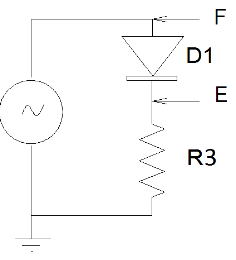
\includegraphics[width=7.5cm]{C-circ}
            \caption{Circuito Utilizado na parte C}
            \label{fig:C-circ}
        \end{figure}
    \subsection{Gráficos}
        \begin{figure} [H] 
            \begin{subfigure}[b]{7cm}  
                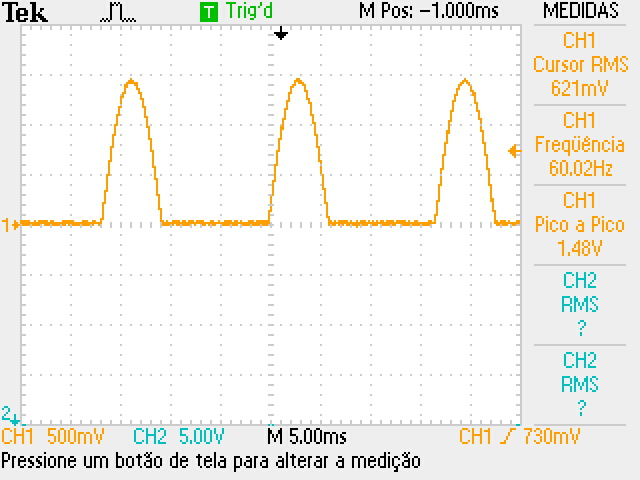
\includegraphics[width=7cm]{C-gnd-e}
                \caption{Nos pontos GND e E}
                \label{fig:C-gnd-e}
            \end{subfigure}
            \begin{subfigure}[b]{7cm}  
                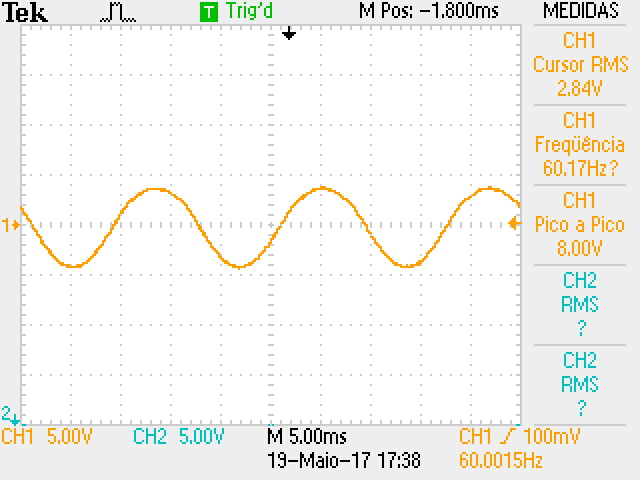
\includegraphics[width=7cm]{C-gnd-f}
                \caption{Nos pontos GND e F}
                \label{fig:C-gnd-f}
            \end{subfigure}
                \caption{Gráfic Uxt no oscilador na parte C}
        \end{figure}
    \subsection{C2}
    \paragraph{Medidas ponto F com o multímetro}

    Obtivemos uma medida de 2,798V. 
    Para o erro associado temos:
    $$\Delta V_f = \frac{0,6\% * 2,798 + 5 * 0,001}{\sqrt{3}} \approx 0,01 V$$
    Reescrevendo, temos:
    $$V_f = (2,80\pm0,01) V$$

    \paragraph{Medidas ponto E com o multímetro} 
    Obtivemos uma medida de 554mV. 
    Para o erro associado temos:
    $$\Delta V_e = \frac{0,6\% * 0,554 + 5 * 0,001)}{\sqrt{3}} \approx 0,005 V$$
    Reescrevendo, temos:
    $$V_e = (554\pm5) mV$$

    \paragraph{Medidas ponto F com o osciloscópio}
    Obtivemos uma medida de $2,84V$. 
    Para o erro associado temos:
    $$\Delta V_f = \frac{3\% |valor medido| + 10\% div + 1mV}{\sqrt{3}}$$
    $$\Delta V_f = \frac{3\% * 2,84 + 10\% * 5 + 0,001}{\sqrt{3}}$$ 
    $$\Delta V_f \approx 0,3 V$$
    Reescrevendo temos: 
    $$V_f = (2,8\pm0,3) V$$

     \paragraph{Medidas ponto E com o osciloscópio}
    Obtivemos uma medida(RMS) de $621mV$.
    Para o erro associado temos:
    $$\Delta V_e = \frac{3\% |valor medido| + 10\% div + 1mV}{\sqrt{3}}$$
    $$\Delta V_e = \frac{3\% * 0,621 + 10\% * 0,5 + 0,001}{\sqrt{3}}$$
    $$\Delta V_e \approx 40 mV$$
    Reescrevendo temos: 
    $$V_e = (620\pm40) mV$$

    \paragraph{Obs} 
    Podemos observar atraves das formas de onda 
    mostradas na tela do osciloscópio 
    (Figuras 7 e 6) que a parte positiva da 
    senóide (Figura 6) se manteve praticamente 
    inalterada, obtendo uma pequena perda 
    referente à queda de tensão necessária 
    para conduzir o diodo, neste caso, 
    polarizado diretamente, enquanto a parte 
    negativa da mesma senóide foi retificada, 
    como observamos na figura 7, devido ao 
    diodo, neste caso, estar polarizado 
    inversamente, bloqueando a passagem de 
    corrente.

    \paragraph{Análise comparativa entre medidas do multímetro e osciloscópio}:


    \begin{tabular}{ | l | l l | }
    \hline 
    Medida\\Instrumento & Multímetro    & Osciloscópio \\ \hline
    Ponto F [V]         & $2,8\pm0,01$  & $2,8\pm0,3$ \\
    Ponto E [mV]        & $554\pm5$     & $620\pm40$ \\
    \hline
    \end{tabular}
    \newline 

    Podemos observar que as medidas do ponto F 
    concordam entre si pois possuem em seus 
    intervalos de incerteza valores comuns 
    entre as medidas do multímetro e 
    osciloscópio, em relação ao ponto E 
    observamos que as medidas são próximas 
    porém não o suficiente para concordarem, 
    temos uma medida acrescida da tolerância 
    máxima para o multímetro de $V_{max} = 559mV$ 
    enquanto para o osciloscópio obtemos uma 
    medida mínima de $V_{min} = 580mV$.

    Note que a tensão efetiva para meia onda deve ser calculada da seguinte forma:
    
    Temos a tensão sobre R3 (Figura \ref{fig:C-gnd-f}) dada por:

    $$V_R(t) = sqrt{2}V_p sen(\omega t), 0 < \omega t < \pi$$
    $$V_{RMS} = \frac{1}{\pi} \int_{0}^{\pi} V_R(t) d(\omega t)$$
    $$V_{RMS} = \frac{sqrt{2}V_p}{\pi} \approx 0,45 V$$

    Dessa forma podemos calcular Vrms tomando $V_p = 1,48 V$ (Figura \ref{fig:C-gnd-e}) obtendo:
    $$V_{rms} = 0,45 * 1,48 \approx 0,650 V$$

    \subsection{C3}

    \paragraph{Visualisação de oscilações}

    A 10Hz de frequência, pudemos observar 
    o LED piscar de forma nítida, a partir 
    de 30Hz não pudemos observar o LED 
    piscando de forma clara e a partir de 
    40Hz a oscilação da luminosidade era 
    praticamente inperceptível.

    Isso se dá ao fato do nosso olho fazer 
    `atualizações` menos de 30 vezes por segundo.